Die Öltröpfchenmethode von Millikan dient dazu, die Elememtarladung $e_0$
zu bestimmen. Dabei werden zerstäubte Öltröpfchen in einen Kondensator gebracht.
Duch die auftretende Reibung bei der Zerstäubung werden die meisten Tröpfchen
mit einem ganzzahligem Vielfachen von $e_0$ geladen.

Aufgrund der Gravitationskraft
\begin{equation}
\vec{F_\su{g}}= m\vec{g}
\end{equation}
werden die Teilchen
so lange nach unten hin beschleunigt, bis sich durch die entegegenwirkende
Reibungskraft
\begin{equation}
\vec{F_\su{R}} = -6\pi r\eta_\su{Luft}\vec{v}
\end{equation}
nach Stokes eine Gleichgewichtsgeschwindigkeit $\vec{v_0}$ einstellt. Es gilt:
\begin{align}
  \vec{F_\su{g}} &= \vec{F_\su{R}} \\
  \frac{4\pi}{3}r^3(\rho_\text{Öl}-\rho_\su{Luft})g &= 6\pi \eta_\su{Luft} r v_0 \\
\end{align}
Hierbei wird der Auftrieb in Luft mit berücksichtigt, welcher der Gravitationskraft
entgegenwirkt. Da die Dichte $\rho_\su{Luft}$ im Vergleich zur Dichte $\rho_\su{Öl}$
jedoch vernachlässigbar klein ist, kann der Auftrieb bei diesem Experiment vernachlässigt
werden und wird nur wegen der Vollständigkeit halber mitgeführt. Für die Masse
$m = \rho \cdot V$ werden die Öltröpfchen als Kugelförmig mit dem Volumen
$V=\sfrac{4}{3}\pi r^3$ angenommen. Für den Radius $r$ folgt damit
\begin{equation}
  r = \sqrt{\frac{9\eta_\su{Luft}v_0}{2g(\rho_\text{Öl}-\rho_\su{Luft})}}.
\end{equation}
Wird nun ein homogenes elektrischen Feld hinzugeschaltet, so ergeben sich die
zwei Fälle aus Abb. \ref{fig:troepfchen}.
\begin{figure}
  \centering
  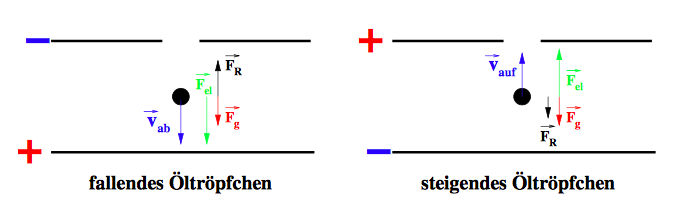
\includegraphics[width=0.8\textwidth]{bilder/troepfchen.png}
  \caption{Kräftegleichgewicht bei eingeschaltetem homogenen elektrischem Feld \cite{503}.}
  \label{fig:troepfchen}
\end{figure}
Wird eine positive Spannung an die untere Platte angelegt, so wirkt
$\vec{F_\su{el}}=q\vec{E}$ zusammen mit der Gravitationskraft nach unten. Das
Tröpfchen bewegt sich mit einer gleichförmigen Geschwindigkeit $v_\su{ab}$,
welche größer als $\vec{v_0}$ ist, nach unten. Damit ergibt sich
\begin{equation}
  \frac{4\pi}{3}r^3(\rho_\text{Öl}-\rho_\su{Luft})g-6\pi \eta_\su{Luft} r v_\su{ab}
  =-qE.
\end{equation}
Wird die Spannung umgepolt, sich wird das Teilchen nach oben beschleunigt und
erfährt die Geschwindigkeit $\vec{v_\su{auf}}$. Da $\vec{F_\su{R}}$ nun nach unten
wirkt folgt damit
\begin{equation}
  \frac{4\pi}{3}r^3(\rho_\text{Öl}+\rho_\su{Luft})g+6\pi \eta_\su{Luft} r v_\su{ab}
  =+qE.
\end{equation}
Für die Ladung $q_0$ ergibt sich dann
\begin{equation}
  q_0 = 3\pi \eta_\su{Luft} \sqrt{\frac{9\eta_\su{Luft}(v_\su{ab}-v_\su{auf})}
  {4g(\rho_\text{Öl}-\rho_\su{Luft})}} \cdot \frac{v_\su{ab}+v_\su{auf}}{E}
  \label{eqn:q0}
\end{equation}
und für den Tröpfchenradius ergibt sich
\begin{equation}
  r = \sqrt{\frac{9\eta_\su{Luft}(v_\su{ab}-v_\su{auf})}
  {2g(\rho_\text{Öl}-\rho_\su{Luft})}}
\end{equation}
Da das Stokesche Gesetzt jedoch nur gilt, wenn die mittlere freie Weglänge $\bar{l}$
in Luft kleiner als die Größe der Öltröpfchen ist. $\bar{l}$ beschreibt die Länge,
die ein Teilchen zurücklegen kann, ohne mit einem anderen Molekül bzw. Teilchen
zusammenzustoßen. Im vorliegenden Versuch ist $\bar{l}$ jedoch größer als die Tröpfchen,
wodurch die Viskosität $\eta_\su{Luft}$ mit
\begin{equation}
  \eta_\su{eff} = \eta_\su{Luft}\bigg(\frac{1}{1+A\frac{1}{r}}\bigg)=\eta_\su{Luft}
  \bigg(\frac{1}{1+B\frac{1}{pr}}\bigg)
  \label{eqn:n}
\end{equation}
korrigiert wird. Für den Cunningham-Korrekturterm gilt $B=6.17\cdot 10^{-3}
\,Torr \cdot \cm$.
Für den Erhalt von $\eta_\su{L}$ wird Grafik \ref{fig:grafik} verwendent. Die
Temperaturen ergeben sich aus Tablle \ref{tab:tabelle} mittels des Thermistor-Widerstands.
\begin{figure}
  \centering
  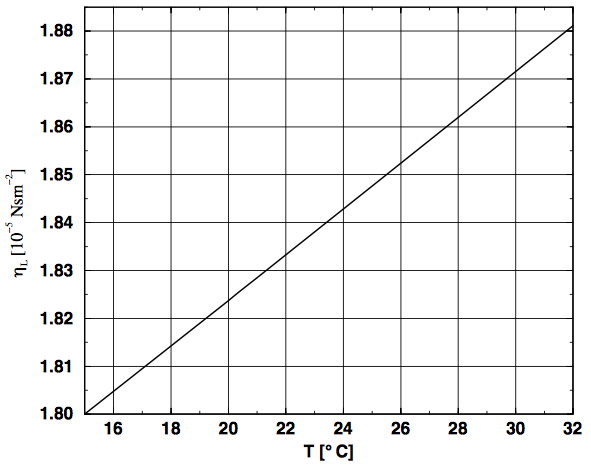
\includegraphics[width=8cm]{bilder/grafik.png}
  \caption{Die Viskosität von Luft als Funktion der Temperatur \cite{503}.}
  \label{fig:grafik}
\end{figure}
Da $\bar{l}$ umgekehrt proportional zum Luftdruck $p$ ist ergibt sich für die
korrigierte Ladung
\begin{equation}
  q^{2/3}=q_0^{2/3} \bigg(\frac{1}{1+B\frac{1}{pr}}\bigg). \label{eqn:q}
\end{equation}
